\documentclass[aspectratio=169]{beamer}

% ===== TEMA =====
\usetheme{metropolis}
\usefonttheme{professionalfonts}

\usepackage{fontspec}
\setmainfont{Carlito}
\setsansfont{Carlito}
\setmonofont{DejaVu Sans Mono}

\usepackage{polyglossia}
\setdefaultlanguage{serbian}

\usepackage{tikz}
\usetikzlibrary{positioning,arrows.meta,shapes.geometric,fit,backgrounds}
\usepackage{booktabs}
\usepackage{array}
\usepackage{graphicx}
\usepackage{colortbl}

% ===== BOJE (identične kao u referentnom šablonu) =====
\definecolor{primarna}{HTML}{6C5CE7}
\definecolor{sekundarna}{HTML}{FF6B81}
\definecolor{tamna}{HTML}{2D3142}
\definecolor{svetla}{HTML}{F5F3FC}

\setbeamercolor{frametitle}{bg=primarna, fg=white}
\setbeamercolor{progress bar}{fg=sekundarna, bg=svetla}
\setbeamercolor{title separator}{fg=sekundarna}
\setbeamercolor{alerted text}{fg=sekundarna}
\setbeamercolor{normal text}{fg=tamna}
\setbeamercolor{block title}{bg=primarna, fg=white}
\setbeamercolor{block body}{bg=svetla, fg=tamna}
\setbeamercolor{palette primary}{bg=primarna, fg=white}

\setbeamertemplate{itemize item}{\color{primarna}\textbullet}
\setbeamertemplate{itemize subitem}{\color{sekundarna}\textendash}

% ===== ORIGINALNE TikZ IKONICE (bez spoljnih slika) =====
\newcommand{\eyeicon}[1][1]{%
\begin{tikzpicture}[scale=#1]
\draw[primarna, line width=2.2pt, fill=svetla] (0,0) ellipse (1.05 and 0.6);
\fill[sekundarna] (0,0) circle (0.32);
\fill[tamna] (0,0) circle (0.13);
\fill[white] (0.09,0.09) circle (0.045);
\end{tikzpicture}%
}
\newcommand{\lockicon}[1][1]{%
\begin{tikzpicture}[scale=#1]
\draw[primarna, line width=4pt, rounded corners=6pt]
  (-0.38,0.1) -- (-0.38,0.42) arc (180:0:0.38) -- (0.38,0.1);
\filldraw[primarna, rounded corners=4pt] (-0.62,-0.62) rectangle (0.62,0.15);
\fill[svetla] (0,-0.18) circle (0.09);
\draw[svetla, line width=2.4pt] (0,-0.18) -- (0,-0.4);
\end{tikzpicture}%
}
\newcommand{\vricon}[1][1]{%
\begin{tikzpicture}[scale=#1]
\draw[primarna, line width=3pt] (-0.9,0.05) -- (-1.3,0.25);
\draw[primarna, line width=3pt] (0.9,0.05) -- (1.3,0.25);
\filldraw[primarna, rounded corners=10pt] (-0.9,-0.4) rectangle (0.9,0.4);
\fill[svetla] (-0.42,0) circle (0.2);
\fill[svetla] (0.42,0) circle (0.2);
\end{tikzpicture}%
}
\newcommand{\giftboxicon}[1][1]{%
\begin{tikzpicture}[scale=#1]
\filldraw[sekundarna, rounded corners=3pt] (-0.6,-0.6) rectangle (0.6,0.3);
\filldraw[primarna] (-0.08,-0.6) rectangle (0.08,0.3);
\filldraw[primarna] (-0.6,-0.05) rectangle (0.6,0.1);
\draw[primarna, line width=2pt] (-0.22,0.3) .. controls (-0.4,0.6) and (-0.05,0.55) .. (0,0.32);
\draw[primarna, line width=2pt] (0.22,0.3) .. controls (0.4,0.6) and (0.05,0.55) .. (0,0.32);
\end{tikzpicture}%
}
\newcommand{\globeicon}[1][1]{%
\begin{tikzpicture}[scale=#1]
\begin{scope}
\clip (0,0) circle (0.9);
\fill[svetla] (-1,-1) rectangle (1,1);
\draw[primarna, line width=1.2pt] (0,0) ellipse (0.38 and 0.9);
\draw[primarna, line width=1.2pt] (-1,0.32) -- (1,0.32);
\draw[primarna, line width=1.2pt] (-1,-0.32) -- (1,-0.32);
\end{scope}
\draw[primarna, line width=2.4pt] (0,0) circle (0.9);
\end{tikzpicture}%
}
\newcommand{\magneticon}[1][1]{%
\begin{tikzpicture}[scale=#1]
\draw[primarna, line width=4pt, line cap=round] (-0.35,-0.55) -- (-0.35,0.05) arc (180:0:0.35) -- (0.35,-0.55);
\draw[sekundarna, line width=4pt, line cap=round] (-0.35,-0.55) -- (-0.35,-0.78);
\draw[sekundarna, line width=4pt, line cap=round] (0.35,-0.55) -- (0.35,-0.78);
\end{tikzpicture}%
}
\newcommand{\sliderseicon}[1][1]{%
\begin{tikzpicture}[scale=#1]
\draw[primarna, line width=2pt] (-0.55,0.32) -- (0.55,0.32);
\fill[sekundarna] (-0.15,0.32) circle (0.09);
\draw[primarna, line width=2pt] (-0.55,0) -- (0.55,0);
\fill[sekundarna] (0.22,0) circle (0.09);
\draw[primarna, line width=2pt] (-0.55,-0.32) -- (0.55,-0.32);
\fill[sekundarna] (-0.05,-0.32) circle (0.09);
\end{tikzpicture}%
}
\newcommand{\shieldicon}[1][1]{%
\begin{tikzpicture}[scale=#1]
\draw[primarna, line width=2.2pt, fill=svetla]
  (0,0.62) -- (0.48,0.4) -- (0.48,-0.12)
  .. controls (0.48,-0.55) and (0.22,-0.75) .. (0,-0.92)
  .. controls (-0.22,-0.75) and (-0.48,-0.55) .. (-0.48,-0.12)
  -- (-0.48,0.4) -- cycle;
\draw[sekundarna, line width=3pt, line cap=round, line join=round]
  (-0.2,-0.15) -- (-0.03,-0.35) -- (0.27,0.1);
\end{tikzpicture}%
}
\newcommand{\signalicon}[1][1]{%
\begin{tikzpicture}[scale=#1]
\fill[sekundarna] (-0.35,-0.35) rectangle (-0.18,-0.1);
\fill[primarna] (-0.09,-0.35) rectangle (0.08,0.05);
\fill[sekundarna] (0.17,-0.35) rectangle (0.34,0.25);
\end{tikzpicture}%
}
\newcommand{\funnelicon}[1][1]{%
\begin{tikzpicture}[scale=#1]
\draw[primarna, line width=2pt, fill=svetla, line join=round]
  (-0.45,0.35) -- (0.45,0.35) -- (0.09,-0.05) -- (0.09,-0.45)
  -- (-0.09,-0.45) -- (-0.09,-0.05) -- cycle;
\end{tikzpicture}%
}
\newcommand{\targeticon}[1][1]{%
\begin{tikzpicture}[scale=#1]
\draw[primarna, line width=2.2pt] (0,0) circle (0.45);
\draw[sekundarna, line width=2.2pt] (0,0) circle (0.25);
\fill[primarna] (0,0) circle (0.09);
\end{tikzpicture}%
}
\newcommand{\oldicon}[1][1]{%
\begin{tikzpicture}[scale=#1]
\draw[primarna, line width=2.2pt, fill=svetla] (-0.5,-0.4) rectangle (0.5,0.4);
\draw[primarna, line width=2.2pt, fill=svetla] (-0.5,0.4) -- (-0.5,0.62) -- (-0.15,0.62) -- (-0.15,0.4);
\fill[sekundarna] (-0.28,-0.1) rectangle (0.28,0.12);
\end{tikzpicture}%
}
\newcommand{\newicon}[1][1]{%
\begin{tikzpicture}[scale=#1]
\draw[primarna, line width=2.2pt, rounded corners=5pt, fill=svetla] (-0.32,-0.65) rectangle (0.32,0.65);
\fill[primarna] (-0.15,0.4) rectangle (0.15,0.5);
\draw[sekundarna, line width=2pt, fill=sekundarna!25] (0.15,-0.05) circle (0.3);
\node[font=\bfseries\tiny, text=sekundarna] at (0.15,-0.05) {\$};
\end{tikzpicture}%
}
\newcommand{\scaleicon}[1][1]{%
\begin{tikzpicture}[scale=#1]
\draw[primarna, line width=2.2pt] (0,0.55) -- (0,-0.55);
\draw[primarna, line width=2.2pt] (-0.55,0.35) -- (0.55,0.35);
\draw[primarna, line width=1.6pt] (-0.55,0.35) -- (-0.72,-0.05) arc (200:340:0.17) -- (-0.38,-0.05) -- (-0.55,0.35);
\draw[primarna, line width=1.6pt] (0.55,0.35) -- (0.38,-0.05) arc (200:340:0.17) -- (0.72,-0.05) -- (0.55,0.35);
\filldraw[primarna] (-0.22,-0.6) -- (0.22,-0.6) -- (0,-0.4) -- cycle;
\end{tikzpicture}%
}
\newcommand{\warningicon}[1][1]{%
\begin{tikzpicture}[scale=#1]
\draw[primarna, line width=2.2pt, fill=svetla, line join=round]
  (0,0.6) -- (0.58,-0.5) -- (-0.58,-0.5) -- cycle;
\fill[sekundarna] (-0.05,0.1) rectangle (0.05,-0.15);
\fill[sekundarna] (0,-0.28) circle (0.05);
\end{tikzpicture}%
}
\newcommand{\fingerprinticon}[1][1]{%
\begin{tikzpicture}[scale=#1]
\foreach \r in {0.2,0.35,0.5,0.65}{
  \draw[primarna, line width=1.6pt] (0,-0.1) ellipse ({\r} and {\r*1.15});
}
\draw[sekundarna, line width=2pt] (0,-0.75) -- (0,0.55);
\end{tikzpicture}%
}
\newcommand{\checkicon}[1][1]{%
\begin{tikzpicture}[scale=#1]
\draw[primarna, line width=2.2pt, fill=svetla] (0,0) circle (0.62);
\draw[sekundarna, line width=3pt, line cap=round, line join=round]
  (-0.28,0) -- (-0.08,-0.25) -- (0.32,0.28);
\end{tikzpicture}%
}
\newcommand{\questionicon}[1][1]{%
\begin{tikzpicture}[scale=#1]
\draw[primarna, line width=2.2pt, fill=svetla] (0,0) circle (0.62);
\node[font=\bfseries\Large, text=sekundarna] at (0,0.02) {?};
\end{tikzpicture}%
}
\title{Data mining u svetu video igara}
\subtitle{Od unapređenja igre do nadzora igrača}
\author{Luka Nedeljković 147/2021}
\date{Računarstvo i društvo}

% mali izvor u donjem desnom uglu slajda
\newcommand{\izvor}[1]{%
  \begin{textblock*}{8cm}(0.6cm,8.6cm)
  {\tiny\color{tamna!60} #1}
  \end{textblock*}%
}
\usepackage[absolute,overlay]{textpos}

% ===== KARTICA (svetla pozadina, kao na dijagramu i GDPR slajdu) =====
\setbeamercolor{cardbg}{bg=svetla, fg=tamna}
\newenvironment{card}{%
\begin{center}
\begin{beamercolorbox}[wd=0.92\paperwidth,sep=10pt,rounded=true,shadow=false]{cardbg}
}{%
\end{beamercolorbox}
\end{center}
}

% ===== GRADIENT FRAME TITLE + LOGO + PROGRESS BAR =====
\makeatletter
\setbeamertemplate{frametitle}{%
  \begin{beamercolorbox}[wd=\paperwidth,ht=2.3cm,dp=0pt]{normal text}
  \end{beamercolorbox}%
  \begin{tikzpicture}[remember picture,overlay]
    \shade[left color=primarna,right color=sekundarna]
      (current page.north west) rectangle ([yshift=-1.15cm]current page.north east);
    \node[anchor=west,text=white,font=\Large\bfseries,inner sep=0pt]
      at ([xshift=0.5cm,yshift=-0.62cm]current page.north west) {\insertframetitle};
    \node[anchor=north east,inner sep=0pt]
      at ([xshift=-0.4cm,yshift=-0.2cm]current page.north east) {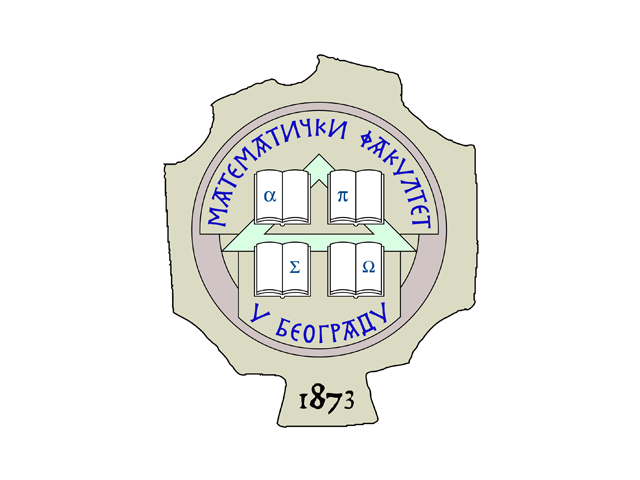
\includegraphics[height=0.9cm]{logo_icon_color.png}};
    \pgfmathsetmacro{\progfrac}{\insertframenumber/\inserttotalframenumber}
    \fill[tamna!12] ([yshift=-1.15cm]current page.north west) rectangle ++({\paperwidth},-0.16cm);
    \fill[sekundarna] ([yshift=-1.15cm]current page.north west) rectangle ++({\progfrac*\paperwidth},-0.16cm);
  \end{tikzpicture}%
}
\makeatother

% ===== SECTION DIVIDER PAGES =====
\setbeamertemplate{section page}{
  \begin{tikzpicture}[remember picture,overlay]
    \shade[left color=primarna,right color=sekundarna,shading angle=35]
      (current page.south west) rectangle (current page.north east);
    \node[anchor=center,text=white,font=\Huge\bfseries,align=center] (secname)
      at (current page.center) {\insertsectionhead};
    \draw[white,line width=0.6pt]
      ([yshift=-0.55cm]secname.south) ++(-3cm,0) -- ++(6cm,0);
  \end{tikzpicture}%
}

\begin{document}

% ---------- NASLOVNA ----------
{
\setbeamertemplate{footline}{}
\usebackgroundtemplate{%
  \begin{tikzpicture}
    \shade[left color=primarna,right color=sekundarna,shading angle=35]
      (0,0) rectangle (\paperwidth,\paperheight);
  \end{tikzpicture}%
}
\begin{frame}[plain]
\begin{center}
\vspace{0.2cm}
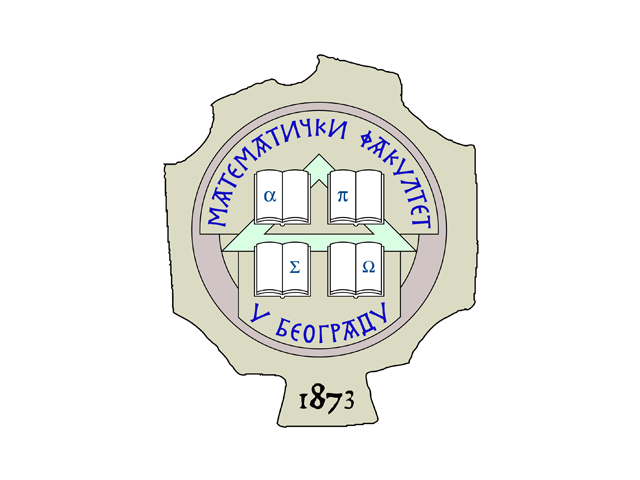
\includegraphics[width=2.3cm]{logo_icon_white.png}\\[0.7cm]
{\usebeamerfont{title}\color{white}\textbf{\inserttitle}}\\[0.5em]
{\usebeamerfont{subtitle}\color{white}\insertsubtitle}\\[0.9em]
{\color{white}\rule{6cm}{0.6pt}}\\[0.9em]
{\small\color{white} Seminarski rad u okviru kursa \insertdate}\\[0.2em]
{\small\color{white} \insertauthor}\\[0.2em]
{\small\color{white} Matematički fakultet, Univerzitet u Beogradu}
\end{center}
\end{frame}
}

% ---------- AGENDA ----------
\begin{frame}{Sadržaj}
\centering
\begin{tikzpicture}[
  card/.style={rectangle, rounded corners=8pt, draw=primarna, fill=svetla, very thick,
               minimum width=6.4cm, minimum height=1.5cm},
  numcirc/.style={circle, fill=primarna, minimum size=0.85cm, text=white,
                  font=\bfseries\large, inner sep=0pt},
  lbl/.style={anchor=west, align=left, text width=4.2cm, text=tamna, font=\large}
]
\node[card] (b1) at (-3.5,2.0) {};
\node[numcirc] at ([xshift=0.95cm]b1.west) {1};
\node[lbl] at ([xshift=1.75cm]b1.west) {Uvod};

\node[card] (b2) at (3.5,2.0) {};
\node[numcirc] at ([xshift=0.95cm]b2.west) {2};
\node[lbl] at ([xshift=1.75cm]b2.west) {Tehnike i primena};

\node[card] (b3) at (-3.5,0) {};
\node[numcirc] at ([xshift=0.95cm]b3.west) {3};
\node[lbl] at ([xshift=1.75cm]b3.west) {Privatnost igrača};

\node[card] (b4) at (3.5,0) {};
\node[numcirc] at ([xshift=0.95cm]b4.west) {4};
\node[lbl] at ([xshift=1.75cm]b4.west) {Etički izazovi};

\node[card] (b5) at (-3.5,-2.0) {};
\node[numcirc] at ([xshift=0.95cm]b5.west) {5};
\node[lbl] at ([xshift=1.75cm]b5.west) {Pravna regulativa};

\node[card] (b6) at (3.5,-2.0) {};
\node[numcirc] at ([xshift=0.95cm]b6.west) {6};
\node[lbl] at ([xshift=1.75cm]b6.west) {Zaključak};
\end{tikzpicture}
\end{frame}

\section{Uvod}

% ---------- UVOD: KONCEPT ----------
\begin{frame}{Šta je data mining u igrama?}
\begin{card}
\begin{center}
\Large Tehnike koje otkrivaju obrasce u ogromnim količinama podataka o \alert{ponašanju igrača}.
\end{center}

\vspace{0.1cm}
\begin{columns}[T]
\begin{column}{0.5\textwidth}
\centering
\oldicon[0.6]\\[0.1em]
\textbf{\large Nekad}
\begin{itemize}
\setlength\itemsep{0.1em}
\item Igra se kupi jednom
\item Transakcija je završena
\item Podatak o igraču -- sporedan
\end{itemize}
\end{column}
\begin{column}{0.5\textwidth}
\centering
\newicon[0.6]\\[0.1em]
\textbf{\large Danas}
\begin{itemize}
\setlength\itemsep{0.1em}
\item \textit{Free-to-play} + mikrotransakcije
\item Igra se prilagođava igraču
\item Podatak o igraču -- poslovna imovina
\end{itemize}
\end{column}
\end{columns}
\end{card}
\izvor{Drachen et al., 2013 -- Game Data Mining}
\end{frame}

% ---------- UVOD: VEZA SA TEMAMA KURSA ----------
\begin{frame}{Veza sa temama kursa}
\begin{card}
\begin{center}
\Large Ista tehnologija koja \textbf{unapređuje} igru omogućava i \alert{nadzor} nad igračem.
\end{center}
\vspace{0.3cm}
\begin{columns}[T]
\begin{column}{0.33\textwidth}
\centering
\lockicon[0.7]\\[0.15em]
{\Huge\color{primarna} 1}\\[0.3em]
\textbf{Privatnost na internetu}\\
{\small vrste podataka, profilisanje}
\end{column}
\begin{column}{0.33\textwidth}
\centering
\scaleicon[0.7]\\[0.15em]
{\Huge\color{primarna} 2}\\[0.3em]
\textbf{Etika}\\
{\small dark patterns, monetizacija}
\end{column}
\begin{column}{0.33\textwidth}
\centering
\warningicon[0.7]\\[0.15em]
{\Huge\color{primarna} 3}\\[0.3em]
\textbf{Internet zavisnost}\\
{\small loot boxovi, kompulsivnost}
\end{column}
\end{columns}
\end{card}
\end{frame}

\section{Tehnike i primena}

% ---------- VRSTE PODATAKA ----------
\begin{frame}{Šta sve igra zna o tebi?}
\begin{card}
\begin{columns}[T]
\begin{column}{0.68\textwidth}
\begin{itemize}
\setlength\itemsep{0.6em}
\item Osnovni podaci: ime, datum rođenja, plaćanje
\item \textbf{Podaci generisani igrom}: kretanje, reakcije, izbori
\item Periferija: miš, dugmad, kod VR -- telo i pogled
\item[$\rightarrow$] \alert{Inferencije}: identitet, starost, pol, emocije, stres
\end{itemize}
\end{column}
\begin{column}{0.32\textwidth}
\centering
\eyeicon[1.3]\\[0.3em]
{\scriptsize\color{tamna!70} igra te ,,gleda`` i kad ti to ne znaš}
\end{column}
\end{columns}
\end{card}
\izvor{Kröger et al., 2023 -- Surveilling the Gamers}
\end{frame}

% ---------- ANALITIKA: 3 STUBA ----------
\begin{frame}{Analitika igrača -- tri poslovna cilja}
\begin{card}
\begin{columns}[T]
\begin{column}{0.33\textwidth}
\centering
\magneticon[0.8]\\[0.15em]
{\Huge\color{primarna} 1}\\[0.2em]
\textbf{Retencija}\\
{\small predviđanje \textit{churn-a} -- kad igrač odustaje}
\end{column}
\begin{column}{0.33\textwidth}
\centering
\sliderseicon[0.8]\\[0.15em]
{\Huge\color{primarna} 2}\\[0.2em]
\textbf{Personalizacija}\\
{\small ponude i težina prilagođene igraču}
\end{column}
\begin{column}{0.33\textwidth}
\centering
\shieldicon[0.8]\\[0.15em]
{\Huge\color{primarna} 3}\\[0.2em]
\textbf{Anti-cheat}\\
{\small statistički neverovatni obrasci}
\end{column}
\end{columns}
\vspace{0.4cm}
\begin{center}
\alert{Problem:} ista infrastruktura koristi se i za profilisanje radi maksimizacije prihoda.
\end{center}
\end{card}
\izvor{Drachen et al., 2013; Bourdoucen et al., 2023}
\end{frame}

% ---------- SISTEM U PRAKSI: DIJAGRAM ----------
\begin{frame}{Kako sistem funkcioniše u praksi}
\centering
\vspace{0.3cm}
\begin{tikzpicture}[
  node distance=0.7cm and 0.7cm,
  box/.style={rectangle, rounded corners, draw=primarna, fill=white, thick,
              minimum width=2.5cm, text width=2.3cm, minimum height=1.2cm, align=center, font=\small},
  arr/.style={-{Stealth[length=2.5mm]}, thick, color=sekundarna}
]
\node[box] (tel) {Telemetrija\\(klik, kupovina, poraz)};
\node[box, right=of tel] (agr) {Agregacija\\i obrada};
\node[box, right=of agr] (seg) {Segmentacija\\igrača};
\node[box, right=of seg] (odl) {Odluka\\u realnom vremenu};

\node[above=0.15cm of tel] {\signalicon[0.65]};
\node[above=0.15cm of agr] {\funnelicon[0.65]};
\node[above=0.15cm of seg] {\sliderseicon[0.55]};
\node[above=0.15cm of odl] {\targeticon[0.65]};

\draw[arr] (tel) -- (agr);
\draw[arr] (agr) -- (seg);
\draw[arr] (seg) -- (odl);
\draw[arr] (odl.south) .. controls +(0,-1.2) and +(0,-1.2) .. (tel.south)
    node[midway, below=0.2cm, font=\scriptsize, align=center] {ponuda ili provera protiv varanja};

\begin{pgfonlayer}{background}
\node[fit=(tel)(agr)(seg)(odl), fill=svetla, rounded corners=16pt, inner sep=0.7cm] {};
\end{pgfonlayer}
\end{tikzpicture}
\vspace{0.7cm}
\izvor{Drachen et al., 2013}
\end{frame}

\section{Privatnost igrača}

% ---------- ZASTO SU PODACI OSETLJIVI ----------
\begin{frame}{Zašto su podaci o igračima osetljivi?}
\begin{card}
\begin{columns}[T]
\begin{column}{0.7\textwidth}
\begin{itemize}
\setlength\itemsep{0.6em}
\item Dugo su igre smatrane ,,bezazlenom`` kategorijom podataka
\item Kröger i saradnici: zaslužuju istu pažnju kao pretraživači i društvene mreže
\item Igrač retko vidi igru kao rizik -- doživljava je kao \textit{zabavu}
\item \alert{Agregacija}: nalozi + plaćanje + platforma $\rightarrow$ detaljan profil
\end{itemize}
\end{column}
\begin{column}{0.3\textwidth}
\centering
\fingerprinticon[0.9]
\end{column}
\end{columns}
\end{card}
\izvor{Kröger et al., 2023}
\end{frame}

% ---------- DECA I BIOMETRIJA ----------
\begin{frame}{Deca i biometrijski podaci}
\begin{card}
\begin{columns}[T]
\begin{column}{0.5\textwidth}
\centering
\shieldicon[0.8]\\[0.15em]
\textbf{\large Deca kao ranjiva grupa}
\begin{itemize}
\item Teže prepoznaju manipulativni dizajn
\item Visoka \textit{lifetime value} za profilisanje
\item Poseban fokus regulative (v. slučaj Epic Games)
\end{itemize}
\end{column}
\begin{column}{0.5\textwidth}
\centering
\vricon[0.9]\\[0.15em]
\textbf{\large VR/AR uređaji}
\begin{itemize}
\item Eye-tracking $\rightarrow$ fokus pažnje, kognitivno stanje
\item Glas $\rightarrow$ emocije, zdravstveni indikatori
\item Akcelerometar $\rightarrow$ fizičke karakteristike
\end{itemize}
\end{column}
\end{columns}
\vspace{0.3cm}
\begin{center}
\alert{Biometrijski podaci se ne mogu ,,resetovati``.}
\end{center}
\end{card}
\izvor{Kröger et al., 2023}
\end{frame}

\section{Etički izazovi}

% ---------- LOOT BOXOVI ----------
\begin{frame}{Loot boxovi: monetizacija zasnovana na podacima}
\begin{card}
\begin{center}
\Large Za razliku od kazina, verovatnoća ishoda je \alert{ista za sve} -- ali \textbf{trenutak ponude} nije.
\end{center}
\vspace{0.3cm}
\begin{columns}[T]
\begin{column}{0.18\textwidth}
\centering
\vspace{0.2cm}
\giftboxicon[1.2]
\end{column}
\begin{column}{0.82\textwidth}
\begin{itemize}
\setlength\itemsep{0.5em}
\item Sistem prepoznaje trenutak kad je igrač najskloniji kupovini
\item Zendle \& Cairns (2018): veza između loot boxova i problematičnog kockanja
\end{itemize}
\end{column}
\end{columns}
\end{card}
\izvor{Zendle \& Cairns, 2018}
\end{frame}

% ---------- DARK PATTERNS TAKSONOMIJA ----------
\begin{frame}{Dark patterns -- tri dimenzije}
\begin{card}
\begin{center}
\small
\renewcommand{\arraystretch}{1.4}
\arrayrulecolor{black!20}
\begin{tabular}{|>{\bfseries}p{3.0cm}|p{6.8cm}|}
\hline
\rowcolor{primarna!18}
\textbf{Dimenzija} & \textbf{Primer} \\
\hline
Vremenska & Ograničene ponude, dnevne nagrade koje vraćaju igrača \\
\hline
Novčana & Konfuzija virtuelnih valuta, loot boxovi \\
\hline
Socijalna & Pritisak vršnjaka, ,,prijatelji su već kupili`` \\
\hline
\end{tabular}
\end{center}
\vspace{0.3cm}
\begin{center}
Najgušće zastupljeni u \alert{mobilnim} igrama -- najprecizniji podaci o kontekstu igrača.
\end{center}
\end{card}
\izvor{Gutiérrez-Manjón et al., 2026}
\end{frame}

\section{Pravna regulativa}

% ---------- GDPR ----------
\begin{frame}{GDPR i video igre}
\begin{card}
\begin{columns}[T]
\begin{column}{0.68\textwidth}
\begin{itemize}
\setlength\itemsep{0.6em}
\item Video igre = digitalna usluga $\rightarrow$ GDPR važi u potpunosti
\item Minimizacija podataka $\times$ poslovni model zasnovan na podacima
\item Član 8: pristanak roditelja za decu mlađu od 16 god.
\item Slučaj Epic Games: ni najveće kompanije to lako ne ispunjavaju
\end{itemize}
\end{column}
\begin{column}{0.32\textwidth}
\centering
\lockicon[1.5]
\end{column}
\end{columns}
\end{card}
\izvor{Uredba (EU) 2016/679 -- GDPR}
\end{frame}

% ---------- BELGIJA: BIG NUMBER ----------
\begin{frame}{Regulacija loot boxova: Belgija, 2018}
\begin{card}
\begin{center}
\Large Belgija -- prva zemlja koja je loot boxove proglasila \alert{nelegalnim kockanjem}.
\end{center}
\vspace{0.4cm}
\begin{columns}[T]
\begin{column}{0.5\textwidth}
\centering
{\Huge\bfseries\color{sekundarna} 82\%}\\[0.3em]
{\small top 100 iPhone igara u Belgiji i dalje nudi nasumičnu monetizaciju}
\end{column}
\begin{column}{0.5\textwidth}
\centering
{\Huge\bfseries\color{sekundarna} 80{,}2\%}\\[0.3em]
{\small od toga -- igre namenjene deci uzrasta 12+}
\end{column}
\end{columns}
\vspace{0.4cm}
\begin{center}
Zaključak: zabrana nailazi na tehničke prepreke -- ponuda se prilagođava po IP adresi.
\end{center}
\end{card}
\izvor{Xiao, 2023 -- Breaking Ban}
\end{frame}

% ---------- ZASTO NACIONALNA REGULATIVA NIJE DOVOLJNA ----------
\begin{frame}{Zašto nacionalna regulativa nije dovoljna}
\begin{card}
\begin{columns}[T]
\begin{column}{0.18\textwidth}
\centering
\vspace{0.3cm}
\globeicon[1.2]
\end{column}
\begin{column}{0.82\textwidth}
\begin{itemize}
\setlength\itemsep{0.6em}
\item Igre su globalne, regulativa je nacionalna
\item Belgija: ponuda se prilagođava po lokaciji
\item SAD (Epic Games): sankcija deluje tek \textit{posle} štete
\item[$\rightarrow$] Potreban \alert{kombinovan pristup}: standardi + regulativa + alati za roditelje
\end{itemize}
\end{column}
\end{columns}
\end{card}
\izvor{Xiao, 2023; Goodstein, 2021}
\end{frame}

\section{Zaključak}

% ---------- ZAKLJUCAK ----------
\begin{frame}{Zaključak}
\begin{card}
\begin{columns}[T]
\begin{column}{0.72\textwidth}
\begin{itemize}
\setlength\itemsep{0.6em}
\item Data mining \textbf{nije problem} -- omogućava bolje igre i anti-cheat
\item Problem: ista infrastruktura bez transparentnosti $\rightarrow$ manipulacija
\item Regulativa postoji, ali zaostaje za industrijom
\item VR/AR čine pitanje sve hitnijim
\end{itemize}
\end{column}
\begin{column}{0.28\textwidth}
\centering
\checkicon[1]
\end{column}
\end{columns}
\end{card}
\end{frame}

% ---------- OTVORENA PITANJA ----------
\begin{frame}{Otvorena pitanja za diskusiju}
\begin{card}
\begin{columns}[T]
\begin{column}{0.72\textwidth}
\begin{itemize}
\setlength\itemsep{0.8em}
\item Može li igrač dati \alert{smislen pristanak} u sistemu projektovanom da bude zabavan?
\item Da li je nacionalna regulativa dovoljna za globalnu industriju?
\item Ko snosi odgovornost kada je granica između dizajna i manipulacije namerno zamagljena?
\end{itemize}
\end{column}
\begin{column}{0.28\textwidth}
\centering
\questionicon[1]
\end{column}
\end{columns}
\end{card}
\end{frame}

% ---------- ZATVARANJE ----------
{
\setbeamertemplate{footline}{}
\usebackgroundtemplate{%
  \begin{tikzpicture}
    \shade[left color=primarna,right color=sekundarna,shading angle=35]
      (0,0) rectangle (\paperwidth,\paperheight);
  \end{tikzpicture}%
}
\begin{frame}[plain]
\begin{tikzpicture}[remember picture,overlay]
  \node[anchor=west, align=left, text=white, font=\small] at ([xshift=1cm]current page.west) {
    Luka Nedeljković 147/2021
  };
\end{tikzpicture}
\begin{center}
\vspace{1.2cm}
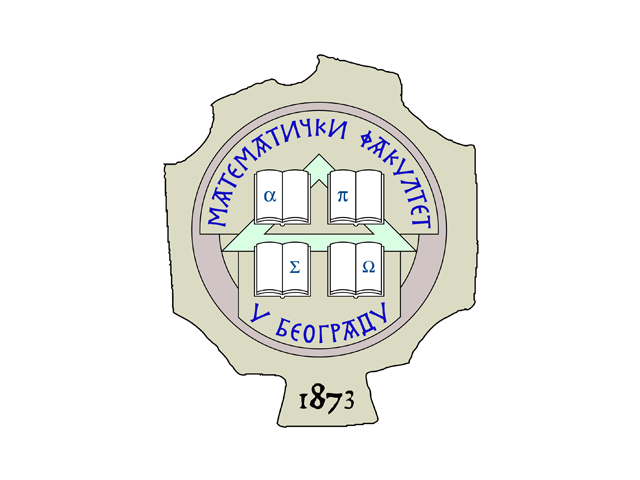
\includegraphics[width=2cm]{logo_icon_white.png}\\[0.7cm]
{\Large\bfseries\color{white} Hvala na pažnji}\\[0.3em]
{\small\color{white} Pitanja?}
\end{center}
\end{frame}
}

\end{document}
